\section{Motivation}
The ability to measure changes in the hemoglobin concentration in skin will enable more personalized patient care which, in turn, will lead to an increase in treatment success rates and a decrease in per-patient costs.

For example, in radiation therapy, a common side effect is a skin-reddening reaction known as erythema, or radiation dermatitis.\cite{McQuestion2006} Depending on the severity of the reaction, erythema can be quite painful and may even prevent the completion of the radiation treatment schedule, thereby reducing the overall treatment efficacy. Unfortunately, since it is a deterministic effect,\cite{Hall2000} with a varying threshold dose and a spectrum of reactions, erythema is impossible to reliably predict in advance. Instead, patients’ responses are monitored by the therapy team over the course of treatment. The current method for monitoring erythema is by visual assessment (VA). VA uses a pre-determined scale to classify the current condition of the skin. If there are too few divisions on the scale (four or less), there is not a sufficient amount of information regarding the patient’s progress from the erythema stage to the next stage of moist desquamation. If there are more than four divisions on the scale, it is difficult to eliminate, or even minimize, the inter- and intra-observer variation, making the results unreliable at best, and preventing any comparison between patients. The implementation of an objective method for measuring skin redness would allow for the treatment team to better manage the reaction, thus improving the treatment’s success rate and the patient’s quality of life.

\section{Light-tissue interactions}
The propagation of light in tissue can be described by three main interactions:\cite{Niemz2007}
\begin{enumerate}
	\item Reflection (and refraction)
	\item Absorption
	\item Scattering
\end{enumerate}

Reflection and refraction occur at the boundary between two materials with different indices of refraction, such as between air and tissue. Neither process can occur if the two materials have equal indices of refraction. For a smooth surface, the light that is reflected at the boundary obeys the law of specular reflection which states that the angle of reflection of a ray of light is equal to the angle of incidence.\cite{Knight2013} Light that is transmitted past the boundary refracts toward the normal as described by Snell's law,

\begin{equation}
n_1 \sin \theta_1 = n_2 \sin \theta_2
\end{equation}

\noindent where $n_1$ and $n_2$ are the indices of refraction of the two materials, $\theta_1$ is the angle of incidence, and $theta_2$ is the angle of refraction.

The amount of light that undergoes either of these two processes can be predicted using Fresnel's equations which require the relative index of refraction ($n_2 / n_1$) and the angle of incidence ($\theta_1$) as their input parameters.CITE PEDROTTI It should be noted that, while most applications approximate the indices of refraction as constants, there is a small wavelength dependence present that should be considered for large wavelength ranges.\cite{Knight2013}

While inside a material, light can either be absorbed or scattered. The probabilities of these two occurrences are based on the optical properties of the material. When an absorption event occurs, the light energy is transferred to a bound electron, elevating it to an excited state.\cite{Jacques2004} Atoms or molecules with excited electronic states can ``discharge'' this energy either through radiative processes such as fluorescence or phosphorescence or, more commonly, through non-radiative processes like vibration. The probability of absorption occurring within an infinitesimal distance $ds$ is $\mu_ads$, where $\mu_a [mm^{-1}]$ is the absorption coefficient. The inverse of the absorption coefficient represents the distance between absorption events. In the case of (elastic) scattering, the energy is absorbed by a free electron that causes acceleration and the emission of a secondary photon with the same frequency.\cite{Jacques2004} The probability of scattering occurring within an infinitesimal distance $ds$ is $\mu_sds$, where $\mu_s [mm^{-1}]$ is the scattering coefficient. The inverse of the scattering coefficient represents the distance between scattering events.

Elastic scattering is isotropic in nature. That is, it is equally probable for the photon to be emitted in any direction. In a homogeneous medium, all directions except the initial photon direction cancel. However, in a medium with many small, suspended particles, another direction may dominate. This can be accounted for with an anisotropy factor ($g$) that is equal to the expectation value (also the average value) of the cosine of the scattering angle. An anisotropy factor of $0$ represents isotropic scattering while a factor of $1$ represents forward scattering. To account for this directionality when modeling light transport in tissue, a reduced scattering coefficient is commonly defined as $\mu_s'=(1-g)\mu_s$ such that its inverse is the distance between isotropic scattering events that produces the same results as the anisotropic scattering.\cite{Gratton2004}

Another helpful quantity is the total reduced attenuation coefficient, $\mu_t'=\mu_a + \mu_s'$ which, when multiplied by an infinitesimal distance, represents the probability of any interaction occuring within that infinitesimal distance. Its inverse is specially termed the ``mean free path'' and represents the average distance between interactions.\cite{Farrell2003}

\section{Modeling of light transport in turbid material}
\subsection{Radiation transport equation and diffusion theory}
The radiation transport equation (RTE), also known as the Boltzmann equation, describes the transfer of neutron particles (in this case, energy in the form of photons) within an infinitesimal volume as a function of time.\cite{Duderstadt1976} It is often expressed as a change in the time- and space-resolved energy radiance, $L(\mathbf{r},\mathbf{\Omega},t)$ with respect to time. This quantity can be determined by investigating the mechanism by which the energy radiance can be gained and lost from the volume in question. When considering the steady-state condition, there is no net change in the energy radiance and the gain terms equal the loss terms.
%\bigskip

\noindent The gain mechanisms are:
\begin{enumerate}
	\item Any photon sources within the volume, $ S(\mathbf{r},\mathbf{\Omega}) $
	\item Photons already within the volume that scatter into the direction of interest,  $\int_{4\pi} L(\mathbf{r},\mathbf{\Omega}) \mu_s(\mathbf{r},\mathbf{\Omega}' \rightarrow \mathbf{\Omega}) d \mathbf{\Omega'} $
	\item Photons that enter into the volume along the direction of interest
\end{enumerate}

\noindent Loss mechanisms include:
\begin{enumerate}
	\item Photons that are absorbed within the volume, $ \mu_a L(\mathbf{r},\mathbf{\Omega}) $
	\item Photons that scatter out of the volume, $ \mu_s L(\mathbf{r},\mathbf{\Omega}) $
	\item Photons that exit the volume
\end{enumerate}
%\bigskip

\noindent A single convection term can be used to account for the photons entering and exiting the volume, $-\mathbf{\Omega}\cdot\nabla L(\mathbf{r},\mathbf{\Omega})$. The combination of all of the terms results in the following equation for the steady-state RTE,\cite{Farrell2003}

\begin{equation}
\label{eq:rte}
\mathbf{\Omega}\cdot\nabla L(\mathbf{r},\mathbf{\Omega}) + (\mu_a + \mu_s) L(\mathbf{r},\mathbf{\Omega}) - \int_{4\pi} L(\mathbf{r},\mathbf{\Omega}) \mu_s(\mathbf{r},\mathbf{\Omega}' \rightarrow \mathbf{\Omega}) d \mathbf{\Omega'} - S(\mathbf{r},\mathbf{\Omega}) = 0
\end{equation}

Solutions to the above equation may be found via intense numerical methods, but they are extremely computationally expensive. As such, a simpler approach is often employed, in which approximations are made that simplify the RTE into a solution-friendly form. In the case of light transport in tissue, the diffusion approximation simplifies the above equation into a single differential equation.
Diffusion theory requires the radiance to be isotropic. This condition is generally met in a semi-infinite medium at a point greater than 1 mfp away from the source or boundaries\cite{Jacques2004} and when $ \mu_a < 0.1\mu_s'$.\cite{Wilson2008} In other words, when the probability of scattering is much greater than the probability of absorption, the direction of the photons is mostly randomized after only a few scattering events, or 1 mfp. The result of these approximations is the diffusion equation as follows,

\begin{equation}
\label{eq:diffeq}
\nabla^2 \cdot \Phi(\mathbf{r}) - \frac{\mu_a}{D}\Phi(\mathbf{r}) = S(\mathbf{r})
\end{equation}

Where $\Phi(\mathbf{r})$ is the energy fluence rate (the integral of the energy radiance over all angles), $D$ is the diffusion constant, $(3\mu_t')^{-1}$, and $S(\mathbf{r})$ is the source term.

The diffusion equation can be solved analytically by applying a set of boundary conditions. In the case of tissue optics, the most common boundary conditions have been developed to account for the mismatch in the index of refraction between the tissue and the air, and the resulting Fresnel reflections from the interior surface of the tissue.

\subsection{Monte Carlo simulations}
Monte Carlo (MC) simulations offer a method of solving the steady-state RTE that is slightly less computationally expensive than traditional numerical methods. It is also useful for confirming solutions for approximations such as diffusion theory. Millions of photons are ``launched'' and their propagation through the medium is determined by the random sampling of probability distributions that represent the absorption and scattering conditions of the medium. This topic is covered thoroughly by Prahl \emph{et al.}\cite{Prahl1989} and Wang \emph{et al.}\cite{Wang1995}

If a single simulation must be run several times with different sets of optical properties, it is useful to adapt the code into what has been termed mono (or “white”) MC.\cite{Alerstam2013} Under this simulation, photons are tracked through a homogeneous scattering, non-absorbing medium. There is no survival weighting in mono MC, so the photons' weights are never modified in the tissue and they are only killed when they scatter too many times (via Russian roulette) or they migrate too far from the region of interest. The total distance traveled by each photon (the pathlength, $s$) in the medium is tracked. When photons are finally scored, their weight is added to a bin for the corresponding total pathlength. The effect of absorption can be introduced after the simulation is complete by multiplying each bin by $\exp(-mua*s)$ and summing over all the bins.

When multiple processors are available on a computer, parallelization is an option for increasing the speed of the MC simulation. In parallel computing, single calculations are performed by each available processor in a computer and the results are collated at the end. Parallelization is only possible if all the calculations are independent of one another (i.e. the order doesn't matter). Since MC is based on stochastic processes, each photon can be treated separately. For example, in a computer with four processors, it is possible to track four photons simultaneously, recording their progress, and collect their results once terminated. This yields a MC simulation that would run four times faster than the original, serial code.

\section{In vivo measurements of tissue optical properties with diffuse reflectance}
\label{sec:diff_refl}
For the purposes of monitoring patient response, \emph{ex vivo} methods for determining tissue optical properties are obviously not appropriate. Therefore, this section will focus solely on a specific subset of available \emph{in vivo} methods – those that require steady-state conditions, as opposed to time resolved systems.

\subsection{Total diffuse reflectance}
\label{sec:total_diff_refl}
The total diffuse reflectance represents the fraction of incident light fluence remitted from the tissue across the entire surface (i.e. it is spatially integrated) at a single wavelength. It can be modelled with the diffusion approximation and is dependent only on the reduced albedo and the relative index of refraction.\cite{Kim2011} The index of refraction for skin has been accurately measured, and a value of 1.4 is typically used for incident light within the visible spectrum.\cite{Kienle1996a} With this information, the albedo of the tissue can be determined from the measured total diffuse reflectance. For a single total diffuse reflectance measurement, there is no way to determine the individual contributions from scattering and absorption. However, if the scattering and mean pathlength are assumed constant, a second measurement, where the absorption coefficient is known or can be approximated, will allow for the determination of the first absorption coefficient. This technique relies on the relationship between the total diffuse reflectance and the exponential of the absorption coefficient and the pathlength. The total diffuse reflectance is generally measured either with an integrating sphere (see Section~\ref{sec:is_theory}) or with an optical system, off-set from the normal to avoid collecting any specular reflectance.

\subsection{Spatially-resolved diffuse reflectance}
\label{sec:spat_diff_refl}
The spatially-resolved diffuse reflectance is the fraction of the incident light remitted at a set of radial distances from the incident light source. It is collected by detection fibers positioned at many (at least two) distances from the source fiber.\cite{Kim2011} To maintain accurate positioning, the source and detection fibers are usually bundled together in a single probe. To improve the signal-to-noise ratio, several probes are used at greater distances (see Figure~\ref{fig:intro-srdr}).

\begin{figure}
	\centering 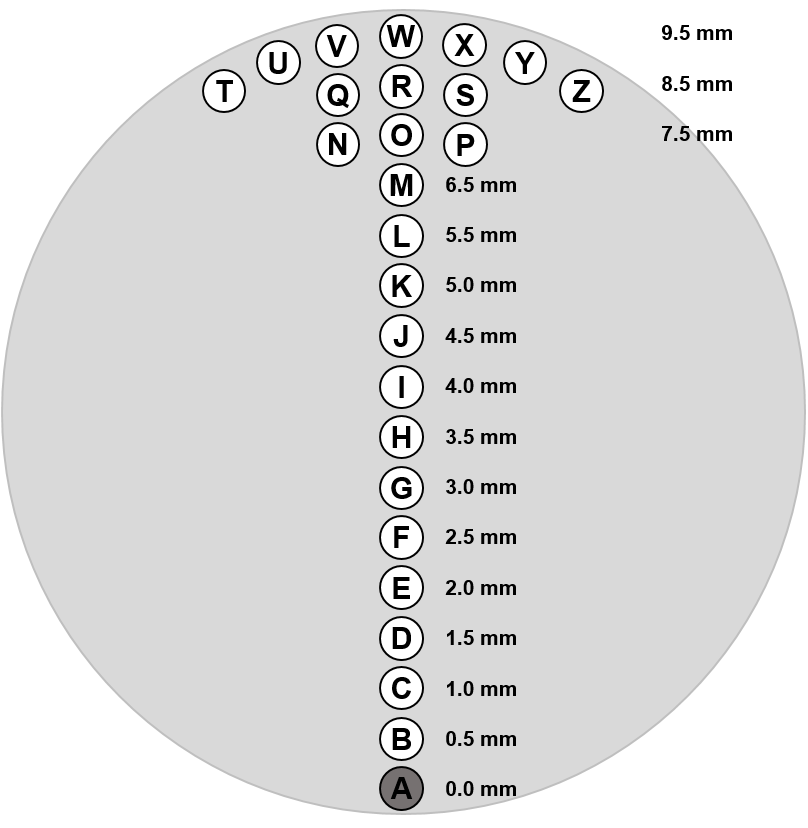
\includegraphics[width=0.5\textwidth]{figures/intro-srdr.png}
	\caption[Probe for spatially-resolved diffuse reflectance]{\label{fig:intro-srdr}A diagram representing the configuration of the optical fibers in the probe. Light enters through fiber “A” (dark grey) and is detected by additional fibers that are placed set distances away (white).}
\end{figure}

Both the absorption and reduced scattering coefficients can be determined with this method. The first step is to determine the effective attenuation coefficient, which is approximated by the terminal slope of the curve of $\ln[r^m R_d(r)] $ as a function of the radial distance. $R_d(r)$ is the measured diffuse reflectance at the radial distance $r$, and $m$ is an empirically determined constant, generally cited as $2$ when diffusion theory applies. After the effective attenuation coefficient has been determined, the measurements from all of the detector probes can be collected to produce the total diffuse reflectance which yields the albedo as described in Section~\ref{sec:total_diff_refl}). Together, these two quantities (the effective attenuation coefficient and the albedo) can be combined to obtain the absorption and reduced scattering coefficient.

\subsection{Spectrally-constrained diffuse reflectance}
\label{spec_diff_refl}
Due to advances in technology, a recently popular method employs a single source-detector pair instead of a spatially-resolved array of detector fibers. In this approach, a broad beam light source is used instead of a single wavelength light source, and the collected signal is resolved into a reflectance measurement at each wavelength. However, this reflectance spectrum is not sufficient to determine the tissue optical properties. Generally, a forward model of the diffusion theory is derived and fit to the obtained reflectance spectrum. Such a model requires both the absorption and reduced scattering coefficient spectra, which can be approximated.

The absorption coefficient is estimated to be the sum of the individual chromophore concentrations $c_i$, multiplied by their respective extinction coefficient spectra $\varepsilon_i(\lambda)$, as follows,

\begin{equation}
\mu_a(\lambda) = \sum_i c_i \varepsilon_i(\lambda)
\end{equation}

The extinction coefficient is the absorption coefficient per molar ($mol/L$) for the medium. These spectra for the majority of chromophores found in human skin (see Section~\ref{sec:skin}) have been well characterized and the chromophore concentrations are included as fitting parameters in the forward model. It is important to include only those chromophores that contribute significantly to the overall absorption within the wavelength range of interest. Including insignificant chromophores will add too many variables to the fitting equation while omitting significant chromophores will yield inaccurate results.

The reduced scattering coefficient for human skin has been well-characterized and follows a wavelength-dependent power law,\cite{Doornbos1999}

\begin{equation}
\mu_s'(\lambda) = a\lambda^{-b}
\end{equation}

As a result, the scaling factor ($a$) and the exponential ($b$) can be included as fitting parameters in the forward model.

\section{Integrating sphere theory}
\label{sec:is_theory}
An integrating sphere is a light delivery and/or collection device. As its name suggests, it is made from a sphere with several ``ports'' cut out of the surface through which light can enter or exit. A typical sphere is shown in Figure~\ref{fig:intro-is_sample}. The inner surface of the sphere is covered with a highly diffuse reflective coating to create what is known as a Lambertian surface. When used as a light delivery device, the light emitted from the irradiation port is uniformly distributed and is isotropic in direction. When used as a measurement device, it is capable of capturing all of the light emitted from the sample area directly below the measurement port. Together, these illumination and measurement qualities make integrating spheres ideal for measuring the total diffuse reflectance (spectra).

\begin{figure}
	\centering 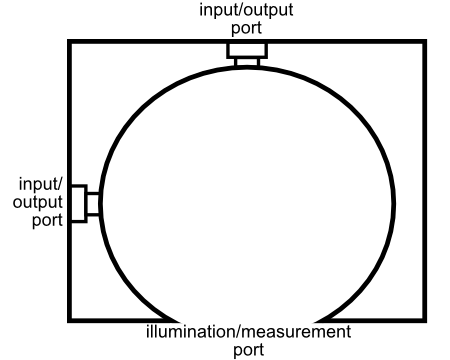
\includegraphics[width=0.5\textwidth]{figures/intro-is_sample.png}
	\caption[Sample integrating sphere diagram]{\label{fig:intro-is_sample}A diagram displaying a common geometry for an integrating sphere. There are two ports for delivering and collecting the light and one port for measuring the reflectance from a sample.}
\end{figure}

\subsection{Relative reflectance and sphere throughput}
The total diffuse reflectance is a relative (as opposed to absolute) reflectance measurement. As such, it requires a characterized reflectance sample known as a reference standard. Measurements performed with the sample of interest are compared (usually as a ratio) to measurements performed with the reference standard. To ensure accurate reflectance measurements, it is important to maintain a consistent throughput, or efficiency within the sphere between the sample and the standard measurements.\cite{Hanssen2002}

The throughput or efficiency of an integrating sphere is the best way of characterizing its performance. It can either be empirically determined or approximated by the following equation,

\begin{equation}
\tau = f_d \frac{\rho_w}{1-\bar{\rho}_w}
\end{equation}

\noindent where $f_d$ is the exchange factor which is equal to the ratio of the total surface area of all the ports to the surface area of the sphere, $\rho_w$ is the actual reflectance of the sphere wall material, and $\bar{\rho}_w$ is the average sphere wall reflectance accounting for the reflectances at the ports.

When the integrating sphere is sufficiently large, a change in the reflectance at one of the ports has a proportionately small effect on the sphere's throughput. Unfortunately, large spheres are not only expensive, but often impractical. For smaller spheres, changes in the sphere throughput between the sample and the reference standard cause what are known as Single Beam Substitution Errors (SBSE) in the total diffuse reflectance measurement.

If the sphere is sufficiently large to allow for an additional ``dummy'' port, a second measurement can be performed to account for SBSE, as shown in Figure~\ref{fig:intro-is_compar}.\cite{Labspherec} The geometry for the first measurement positions the sample directly opposite the light source and the reference standard at the dummy port. This is the primary reflectance measurement. The geometry for the second measurement positions the reference standard directly opposite the light source and the sample at the dummy port. This represents the background correction factor. Under this experimental design, the sphere throughputs and average reflectances are equal for the two measurements.

\begin{figure}
	\centering 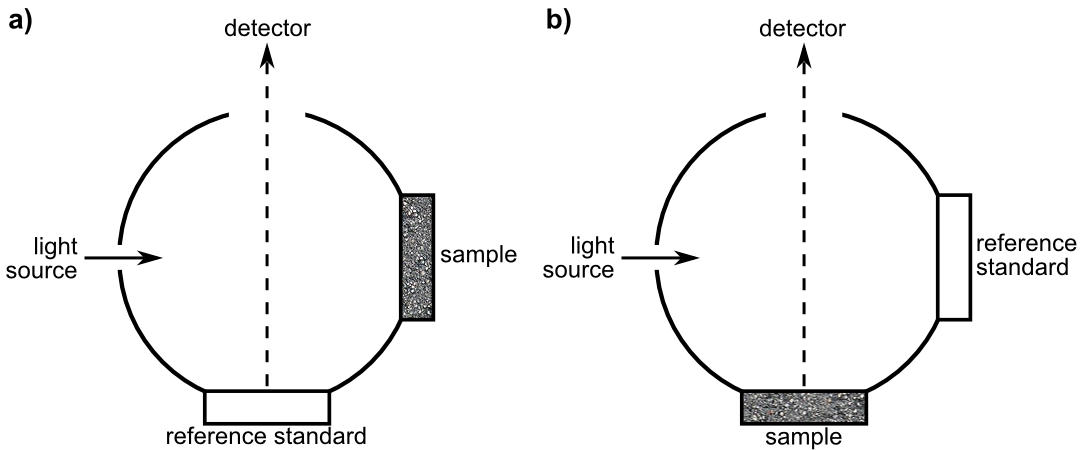
\includegraphics[width=1.0\textwidth]{figures/intro-is_compar.png}
	\caption[The comparison method for measuring sample reflectance]{\label{fig:intro-is_compar}To ensure a constant throughput in the sphere between sample and reference measurements, a dummy port can be added to sufficiently large spheres.}
\end{figure}

If the sphere is too small to permit a second port, the SBSE must be corrected mathematically or empirically. Of these two options, the empirically approach is preferred as a mathematical solution would be extremely complex and only accurate if precise values for parameters such as port fractions and reflectances were provided. For a given sphere, measurements are performed on a set of characterized reflectance standards covering the range of reflectances expected from the samples. By comparing the observed reflectances to the expected ones, a correction factor equation or a lookup table can be produced. REFERENCE TO PAPER \#1?

\subsection{Integrating sphere design}
When creating a new integrating sphere, there are several major designs considerations that must be optimized to minimize measurement error. The first of such options is the sphere size which cannot be determined until the total surface area of all of the ports is determined. Ports intended for coupling with optical fibers will have a set surface area while the size of the detection/illumination port(s) will depend on the use of the sphere. Once the total surface area of the ports has been determined, the sphere size can be calculated based on the rule of thumb that the resulting exchange factor be less than 5\%.\cite{Labsphereb} Spheres that exceed this ratio no longer display some of the desired characteristics such as the isotropy of the light within the sphere.

The next consideration is the material of the sphere, or the sphere's internal coating. Spheres can be created from a highly reflective material such as Spectralon, or they can be produced with a standard plastic material and subsequently coating on the inside with a highly reflective paint, such as barium sulfate. In either case, it is extremely important that the interior surface of the sphere have as high a reflectance as possible, ideally greater than 94\%. This material should also be matte or diffuse in nature, not glossy to produce the desired scattering that creates the isotropic illumination.

The final consideration for the integrating sphere would be the geometry of the ports. With few exceptions, it is important for light from the input port to not be directly incident on the output port. To accomplish this, the numerical aperture of the optical fibers connected to the ports and the overall sphere geometry should be considered. If physical positioning of the ports cannot accomplish this task,  wall projections into the center of the sphere, known as baffles, can be added. Baffles are not ideal for smaller spheres as they introduce inhomogeneities to the smooth inner surface of the sphere that affect the isotropic characteristic. Once this requirement has been satisfied, the illumination geometry can be decided. The two most popular setups are: (1) diffuse-direct (d/0\degree), where incident light is first incident on the sphere wall and the detection port is directly opposite the output port, and (2) direct-diffuse (0\degree/d), where the incident light is first incident on the detection port and the output port is focused on a portion of the inner sphere wall.\cite{Springsteen1998}

\section{Human skin}
\label{sec:skin}
Human skin consists of three main layers: the epidermis, the dermis, and the subcutaneous layer.\cite{Fodor2011a} The epidermis is the top-most layer of skin. As shown in Figure~\ref{fig:intro-skin_layers}, Keratinocytes (skin cells) are produced at the deepest section of the epidermis in the stratum basale and migrate toward the surface, through the statum spinosum and the stratum granulosum to the stratum corneum, losing their internal structures and organelles during the process. The stratum corneum on the skin surface consists of dead, mature keratinocytes which are easily shed. Also found in the epidermis are melanocytes, the melanin-producing cells which are majorly responsible for skin color. The average epidermal thickness is 0.1 mm.\cite{Yang2009}

\begin{figure}
	\centering 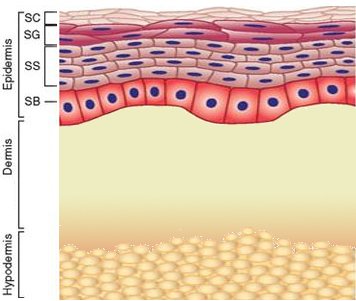
\includegraphics[width=0.5\textwidth]{figures/intro-skin_layers.jpg}
	\caption[Cross-section of layers of human skin]{\label{fig:intro-skin_layers}The three main layers of skin: The epidermis, the dermis, and the subcutaneous layers. Cells of the epidermis begin at the stratum basale (SB) and migrate through the stratum spinosum (SS) and stratum gradulosum (SG) to the stratum corneum (SC). Modified with permission: \textcopyright David J. Wong (\url{http://www.stembook.org}), \href{http://creativecommons.org/licenses/by-sa/3.0/}{CC-BY-SA-3.0}.\cite{Wong2009}}
\end{figure}

The second layer of skin is the dermis. It contains mostly collagen and elastin fibers but is also the location of capillaries and some nerves. The average dermal thickness is approximately 1.5 mm but can vary widely depending on the site.

Below the skin is the subcutaneous layer, also known as the hypodermis or subcutis. The thickness of this layer varies greatly because this is the layer that contains subcutaneous fat. This is also the location of the majority of superficial veins which can occasionally be visible at the surface. A representative thickness for this layer is 5 mm.

Within the visible spectrum (400-750 nm), the dominant chromophores found in skin are: oxy- and deoxy-hemoglobin, and melanin. The relative absorption coefficients for these three chromophores is shown in Figure~\ref{fig:intro-skin_chromophores}. While water does account for roughly 70\% (w/w) of human tissue,\cite{Nakagawa2010} its absorption below 700 nm is negligible. Similarly, beta-carotene (in the epidermis) and bilirubin (in the dermis) do not contribute at wavelengths above 450nm. They are also found in relatively small concentrations in healthy human skin. Although it contribution is small, there is a significant amount of absorption by the structural components of skin.\cite{Bargo2005}

\begin{figure}
	\centering 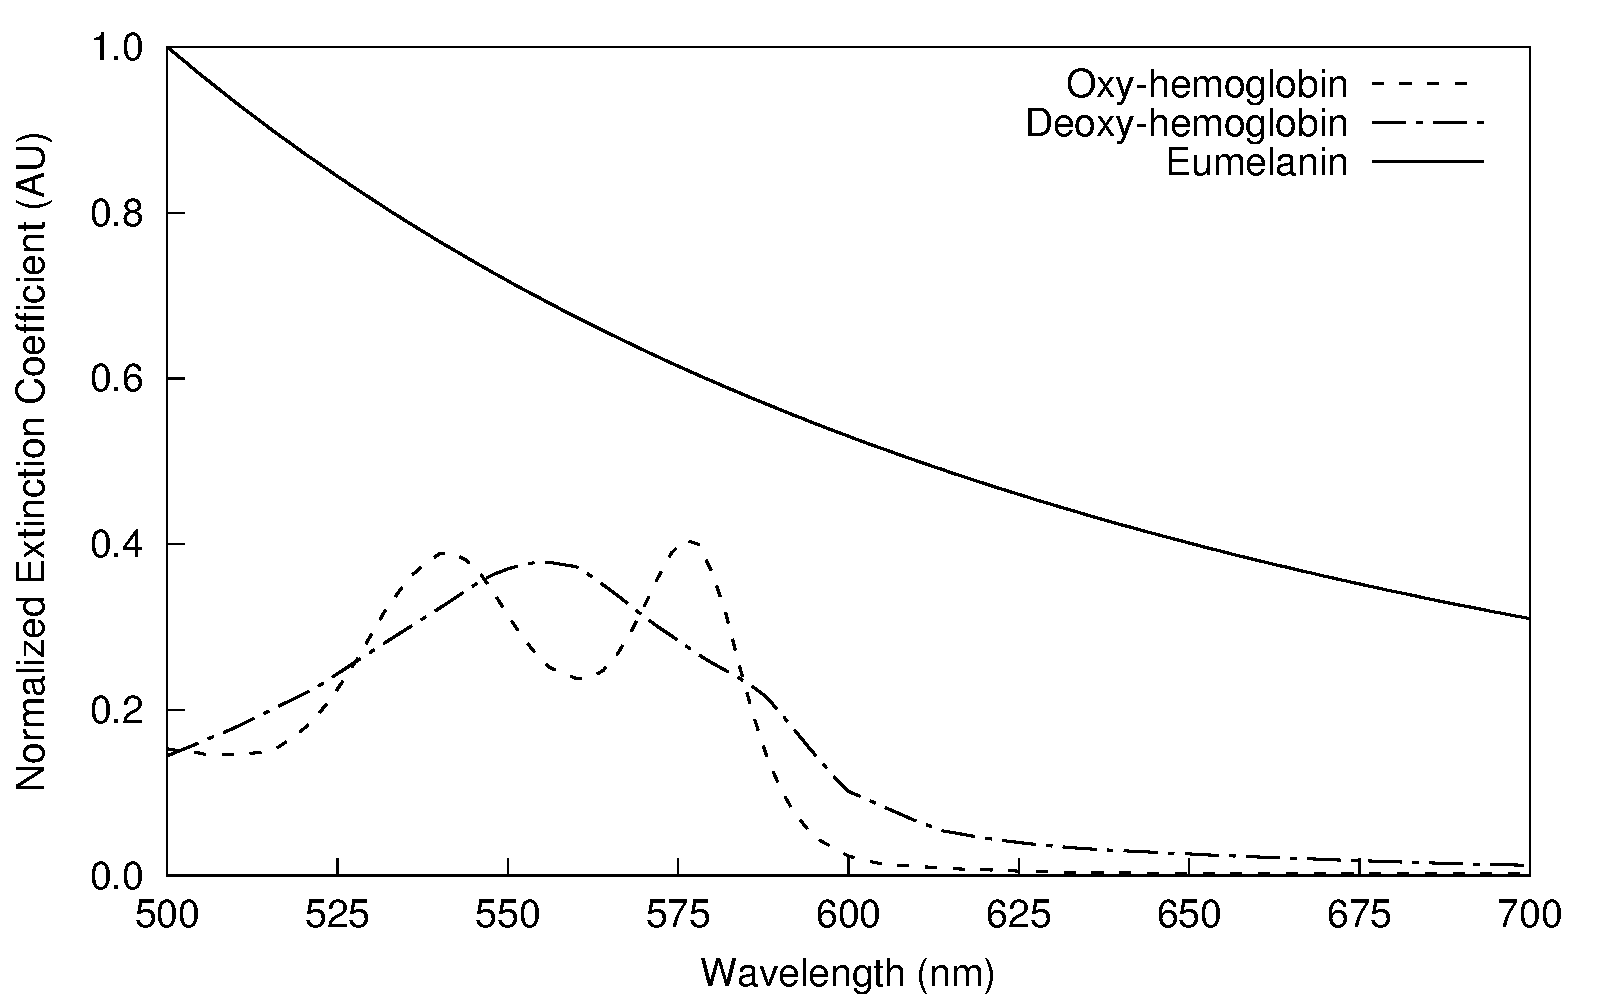
\includegraphics[width=0.8\textwidth]{figures/intro-skin_chromophores.png}
	\caption[The major chromophores of skin within the visible light spectrum]{\label{fig:intro-skin_chromophores}The major chromophores found in skin within the visible light spectrum are oxy- and deoxy-hemoglobin and melanin.}
\end{figure}

Perfusion is the process of delivering blood to capillaries, such as those in the dermal layer of the skin. Changes to the vasculature impact the blood flow within the skin that, in turn, changes the physical appearance at the surface. When the blood vessels narrow, less blood is present in the dermal layer of the skin. This process is known as vasoconstriction and results in a perceived blanching of the skin. When the blood vessels expand in a process known as vasodilation, more blood is present in the skin, which appears redder to the human eye.

It is important to note that, as illustrated in Figure~\ref{fig:intro-skin_chromophores}, both oxy- and deoxy-hemoglobin have low absorption in the red region of the visible spectrum, but have significant absorption within the green/yellow region. Therefore, when vasodilation occurs, the skin does not appear redder because more red light is being reflected. Rather, it is because less of the other colors are reflected. Similarly, when vasoconstriction occurs, more green and yellow light is reflected, contributing to a whiter appearance as white light is a collection of all of the colors within the visible spectrum.

In regards to the ratio of the two hemoglobin chormophores during these two processes, McNaulty \emph{et al.} determined that the tissue oxygen saturation ($StO_2$) is related to blood flow.\cite{McNulty2011} Therefore, more oxy-hemoglobin is present during vasodilation and less is present during vasoconstriction.



\section{Thesis proposal}
Currently available commercial systems for monitoring erythema rely on total diffuse reflectance spectroscopy. As a result, they can only provide measurements in the form of a skin reddness scale (or ``erythema index''). Such an index is only capable of detecting when skin is more or less red compared to some baseline measurement, and it cannot account for changes in non-hemoglobin chromophores.

Other clinical systems rely on a spatially-fixed spectrally-constrained diffuse reflectance approach. Such systems are capable of accounting for changes in the non-hemoglobin chromopores but are difficult to use and are sensitive to positioning errors.

A combination of the two approaches will result in a user-friendly system capable of accounting for all chromophore concentration changes. Thus, a spectrally-constrained model to interpret the total diffuse reflectance spectra obtained with an integrating sphere is proposed. In Chapter~2, a paper is presented that outlines the elements of such a system and how its response should be characterized. In Chapter~3, a paper proposing a spectrally-constrained model for interpreting the spectra obtained with the established system is presented. Special consideration is paid to the necessary corrections required when the total diffuse reflectance spectrum is collected instead of the standard fixed-position diffuse reflectance spectrum. The system and model are then combined in Chapter~4 and used to monitor the skin redness of patients undergoing intensity-modulated radiation therapy (IMRT) for cancers of the head and neck. The results are used to outline the proper implementation of qualitative analysis in a study comparing two treatment interventions or management regimens. Such additional consideration is necessary due to the large daily variation in the hemoglobin concentration in skin. Along with the skin redness measurements, weekly TLD readings were performed to confirm the skin dose in the measurement region. This data was later deemed to have its own intrinsic value, and was used to determine TLD placement and positioning reproducibility in Chapter~5.